%************************************************
\section{Simulation Runtime} % (fold)
\label{sec:simulation_runtime}
%************************************************
The aim of this component is to enable the simulation user to interact with the 3D model, created using the simulation designer. As observed in the related work, some of the projects used a 3D model to represent the environment (\ref{sec:simact}, \ref{sec:ubiwise}, \ref{sec:tatus}) and have built the frameworks on various game engines. A game engine represents a software framework designed for the creation and development of video games. Michael Lewis and Jeffrey Jacobson \cite{lewis2002game} argue for the power of game engines: ''The most sophisticated, responsive interactive simulations are now found in the engines built to power games''. Moreover, they argue for the usefulness of game engines in scientific research: ''There are probably as many potential applications for game engines as there are research problems requiring medium-fidelity 3D simulation or high-fidelity interactive graphics. Our hope is to raise awareness of the high-power/lowcost alternative game engines can offer''.\\

Our design proposal for the simulation runtime is to use a game engine as a starting point. There is wide range of available game engines written in different programming languages, some open-source, others proprietary, most of them providing out of the box components to be reused for specific programming tasks. In conclusion, game engines can fit the various needs and programming experience of the research group designing a simulation for research. The overall design solution we provide based on a game engine is not tied to a certain implementation, but it uses general concepts that can be found in most modern game engines.\\

To conclude this section, we will briefly discuss the architecture of a game engine and present the most important concepts used in game engines which are relevant for this work.\\

%************************************************
\subsection{Architecture of a Game Engine}\label{subsec:game_engine_architecture}
%************************************************
Analysing the game engine's structure depicted in Figure \ref{fig:game_engine_structure}, we can deduct that the game engine renders the virtual environment represented as a 3D or 2D model, while the game code is the custom behaviour for a specific game. Moreover, support for client-server behaviour (usually for multi-player games) can be implemented through the network code module. The fact that the game engine runs at a high-level within an operating system, above the system drivers, makes the client modules platform-independent. The game engine works just like an interpreter, running the same client code (game) on all the supported platforms. Hence, the game engine comes as a solution for requirement \ref{us:3}.\\
\begin{figure}[H]
	\centering
	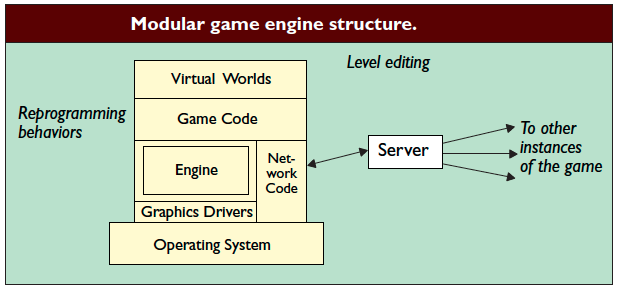
\includegraphics[width=\linewidth]{gfx/Chapter3/game_engine_structure}
	\caption{Modular game engine structure from \cite{lewis2002game}}
	\label{fig:game_engine_structure}
\end{figure}

''A game engine includes all elements in Figure \ref{fig:game_engine_architecture} that have no effect on actual content, that is, everything indicated by dashed lines plus an event loop'' \cite{shantz1998designing}. Therefore, the core features provided by a game engine include a graphics module (rendering engine for 3D graphics), input control (communication with peripherals like mouse, keyboard, joystick, etc), dynamics (e.g. approximate simulation of certain physical systems, such as rigid body dynamics, fluid dynamics, etc), sound. The \emph{event handler}, \emph{game logic} and \emph{level data} (environment model) are client modules that are used to implement a certain type of game / simulation.\\
\begin{figure}[H]
	\centering
	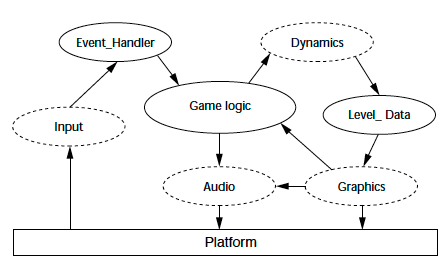
\includegraphics[width=\linewidth]{gfx/Chapter3/game_engine_architecture}
	\caption{Game engine architecture from \cite{shantz1998designing}. The components marked with dashed lines, are contained within the game engine, while the one marked with solid lines (except for the platform) represent client code.}
	\label{fig:game_engine_architecture}
\end{figure}
% subsection architecture_of_a_game_engine (end)

%************************************************
\subsection{Game Engine Concepts}\label{subsec:game_engine_concepts}
%************************************************
The graphics module (renderer) interprets the environment model as a \emph{\textlabel{scene graph}{scene_graph}}, depicted in Figure \ref{fig:scene_graph}. The scene graph is a tree-structured graph, representing the programmatic model of the environment inferred from the simulated environment's virtual model created with the Simulation Designer \ref{sec:simulation_designer}. Besides the information required for rendering, some nodes should carry the Ego metadata the system designer might have attached in the design process. The nodes in the scene graph are the entities used in programming tasks carried out within the game logic.
\begin{figure}[H]
	\centering
	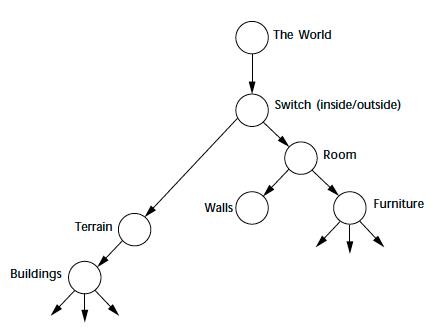
\includegraphics[width=\linewidth]{gfx/Chapter3/scene_graph}
	\caption{Scene graph \cite{shantz1998designing}}
	\label{fig:scene_graph}
\end{figure}

''Missing from Figure \ref{fig:scene_graph} is the \emph{\textlabel{camera}{camera}}, an object not part of the scene graph [...]. The root of a scene graph is attached to a camera when both are initialized''\cite{shantz1998designing}. Using the information of a certain camera (position and orientation) and the scene graph, the renderer computes how to draw the 3D scene graph to the 2D screen. This is what the user sees on the computer screen as the game unfolds. We can think of a camera positioned at a certain point and having a certain direction as the user's field of vision, displaying what the user would actually see if she/he would be located as such. In a game, there can be multiple cameras, providing different perspectives.\\

The mathematical computations used by the graphics engine are all based on absolute or relative coordinates of the entities. Coordinates represent a location in a coordinate system. 3D game engines use a 3D coordinate system. As illustrated in Figure \ref{fig:3d_coordinates_system}, coordinates are relative to the origin at (0, 0, 0). In 3D space, we need to specify three coordinate values to locate a point: X (right), Y (up), Z (towards us). Similarly, -X (left), -Y (down), -Z (away from us).\\
\begin{figure}[H]
	\centering
	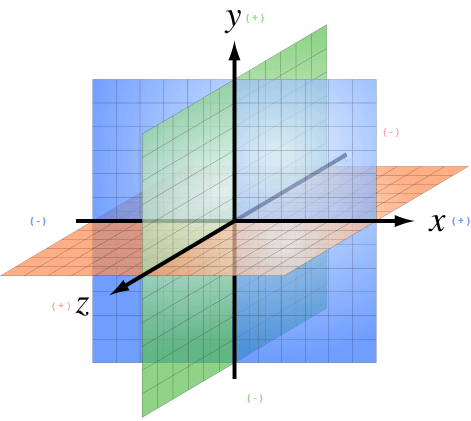
\includegraphics[width=\linewidth]{gfx/Chapter3/coordinate_system}
	\caption{A 3D coordinate system \cite{jme3_terminology:online}}
	\label{fig:3d_coordinates_system}
\end{figure}

As mentioned above, the origin is the central point in the 3D world, where the three axes meet, at the coordinates (0, 0, 0). A coordinate represents a location within the given coordinate system. To represent a direction, game engines use the concept of vectors. A \emph{\textlabel{vector}{vector}} has a length and a direction, just like an arrow in 3D space. A vector starts at a coordinate (x1, y1, z1) or at the origin, and ends at the target coordinate (x2, y2, z2). Backwards directions are expressed with negative values.\\

With this concrete information, let's take a step back to reflect on the concept of a camera. As we have already mentioned, the camera is made up by a location and a direction. The region of space that appears on the computer screen at a certain point is called the \emph{\textlabel{view frustum}{view_frustum}}. This is basically the \emph{field of vision} of the active camera and it is illustrated in Figure \ref{fig:view_frustum}.\\
\begin{figure}[H]
	\centering
	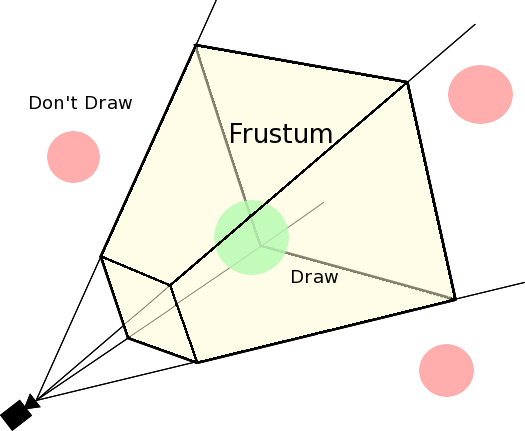
\includegraphics[width=\linewidth]{gfx/Chapter3/view_frustum}
	\caption{View Frustum or Field of Vision}
	\label{fig:view_frustum}
\end{figure}

So, the camera contains both information about the location and direction of the camera within the 3D world, as well as information about the view frustum of the camera. The game engine uses the camera and the scene graph to determine which objects to draw and which not to. This concept is called \emph{culling}.\\

Another useful term in game engines is the \emph{\textlabel{bounding volume}{bounding_volume}}. 3D objects can have irregular forms, other that basic 3D geometrical shapes. To aid mathematical computation, they are wrapped in a bounding volume which pragmatically represents the object as a sphere, cube, cylinder, etc. The bounding volume is then used to compute physical interactions (where physical objects collide, push and bump off one another), and non-physical collisions (mathematical intersections).\\

Finally, the concept of \emph{\textlabel{ray casting}{ray_casting}} is useful to compute distances. Imagine the ray casts a line starting in a certain point of the 3D space having either a finite or infinite length. This ray can be used to determine what objects in the 3D space it intersected. With this information we can determine distance to certain objects.\\
% subsection game_engine_concepts (end)

%************************************************
\subsection{Simulation Runtime Summary}\label{subsec:simulation_runtime_summary}
%************************************************
To summarise, based on the research presented in this section we decided to base the simulation runtime on a game engine. In the last part of this section we have presented the most relevant concepts for our work in the game engines terminology. The \ref{scene_graph} represents a programmatic data structure of the simulated 3D world. The field of vision within the 3D space is provided by the \ref{camera} based on the \ref{view_frustum}, which is computed using the current \ref{vector} (location and direction) of the \ref{camera}. To aid mathematical computations, the 3D representations of objects are wrapped in a bounding volume, regulating their form to basic 3D geometrical shapes. Last, to compute distances the concept of \ref{ray_casting} comes in handy.\\

The design of the following components will use the game engine components and terminology presented in this section.
% subsection simulation_runtime_summary (end)

% \subsection{The Monitoring Service}\label{subsec:monitoring_service}
% \subsection{The API}\label{subsec:api}
% \subsection{The ContextClient}\label{subsec:context_client}
% section simulation_runtime (end)